\documentclass[12pt, a4paper]{article}
\usepackage[spanish]{babel}
\usepackage[utf8]{inputenc}
\usepackage{graphicx}
\usepackage{geometry}
\usepackage{fancyhdr}
\usepackage{float}
\usepackage{titling}
\usepackage{hyperref}
\usepackage{url}

% Márgenes
\geometry{a4paper, margin=2.5cm}

% Encabezado y pie de página
\pagestyle{fancy}
\fancyhf{}
\rhead{
\includegraphics[height=1.2cm]{images/logo-usm.png}}
\lhead{Grupo 19\\Visualización de Datos}
\rfoot{Página \thepage}

% Configuración del logo en portada
\pretitle{
  \begin{center}
  \vspace{1cm}
  
\includegraphics[width=0.5\textwidth]{images/logo-usm.png}\\
  \vspace{1.5cm}
  \LARGE
}
\posttitle{\end{center}}

% Título del informe
\title{Informe: Tecnología en la Vida Cotidiana}
\author{Felipe Campaña, Javier Gómez, Matias Elgueta}
\date{\today\\[2cm]}

\begin{document}
\maketitle

% ---------------------------------------------------------------------------------
\section*{Criterios de Selección}
\begin{itemize}
    \item Criterio 1: Porcentaje de uso de internet en el mundo
    \item Criterio 2: Porcentajes de contratación de fibra en el mundo (Top 10)
    \item Criterio 3: Horas en redes sociales por país
    \item Criterio 4: Evolución de clientes de Telecomunicación
    \item Criterio 5: **
    \item Criterio 6: **
\end{itemize}

% ---------------------------------------------------------------------------------
\section*{Análisis por Integrante}

% ===================== FELIPE CAMPAÑA =====================
\subsection*{Integrante 1: Felipe Campaña}

\subsubsection*{Criterios Seleccionados}
\begin{itemize}
    \item Porcentaje de uso de internet en el mundo.
    \item Porcentajes de contratación de fibra en el mundo (Top 10).
\end{itemize}

\subsubsection*{Justificación: Contratación de Fibra Óptica Fija}
Este indicador representa cuántas personas por cada 100 habitantes tienen acceso a Internet mediante conexiones de alta velocidad y calidad. 

\begin{itemize}
    \item Evalúa el nivel de infraestructura tecnológica en cada país.
    \item Refleja el grado de modernización digital más allá de la simple conectividad.
    \item Relacionado con la capacidad de ofrecer servicios como streaming, teletrabajo, etc.
\end{itemize}

\subsubsection*{Justificación: Acceso a Internet en la Población}
Este indicador señala el porcentaje de personas que utilizan Internet, sin importar el tipo de conexión.

\begin{itemize}
    \item Entrega una visión inclusiva del uso digital básico en cada país.
    \item Identifica regiones con barreras fundamentales de conectividad.
    \item Refleja impacto de políticas públicas y accesibilidad económica.
\end{itemize}

\subsubsection*{Gráfico 1: Uso de internet de las personas en el mundo}
\begin{figure}[H]
    \centering
    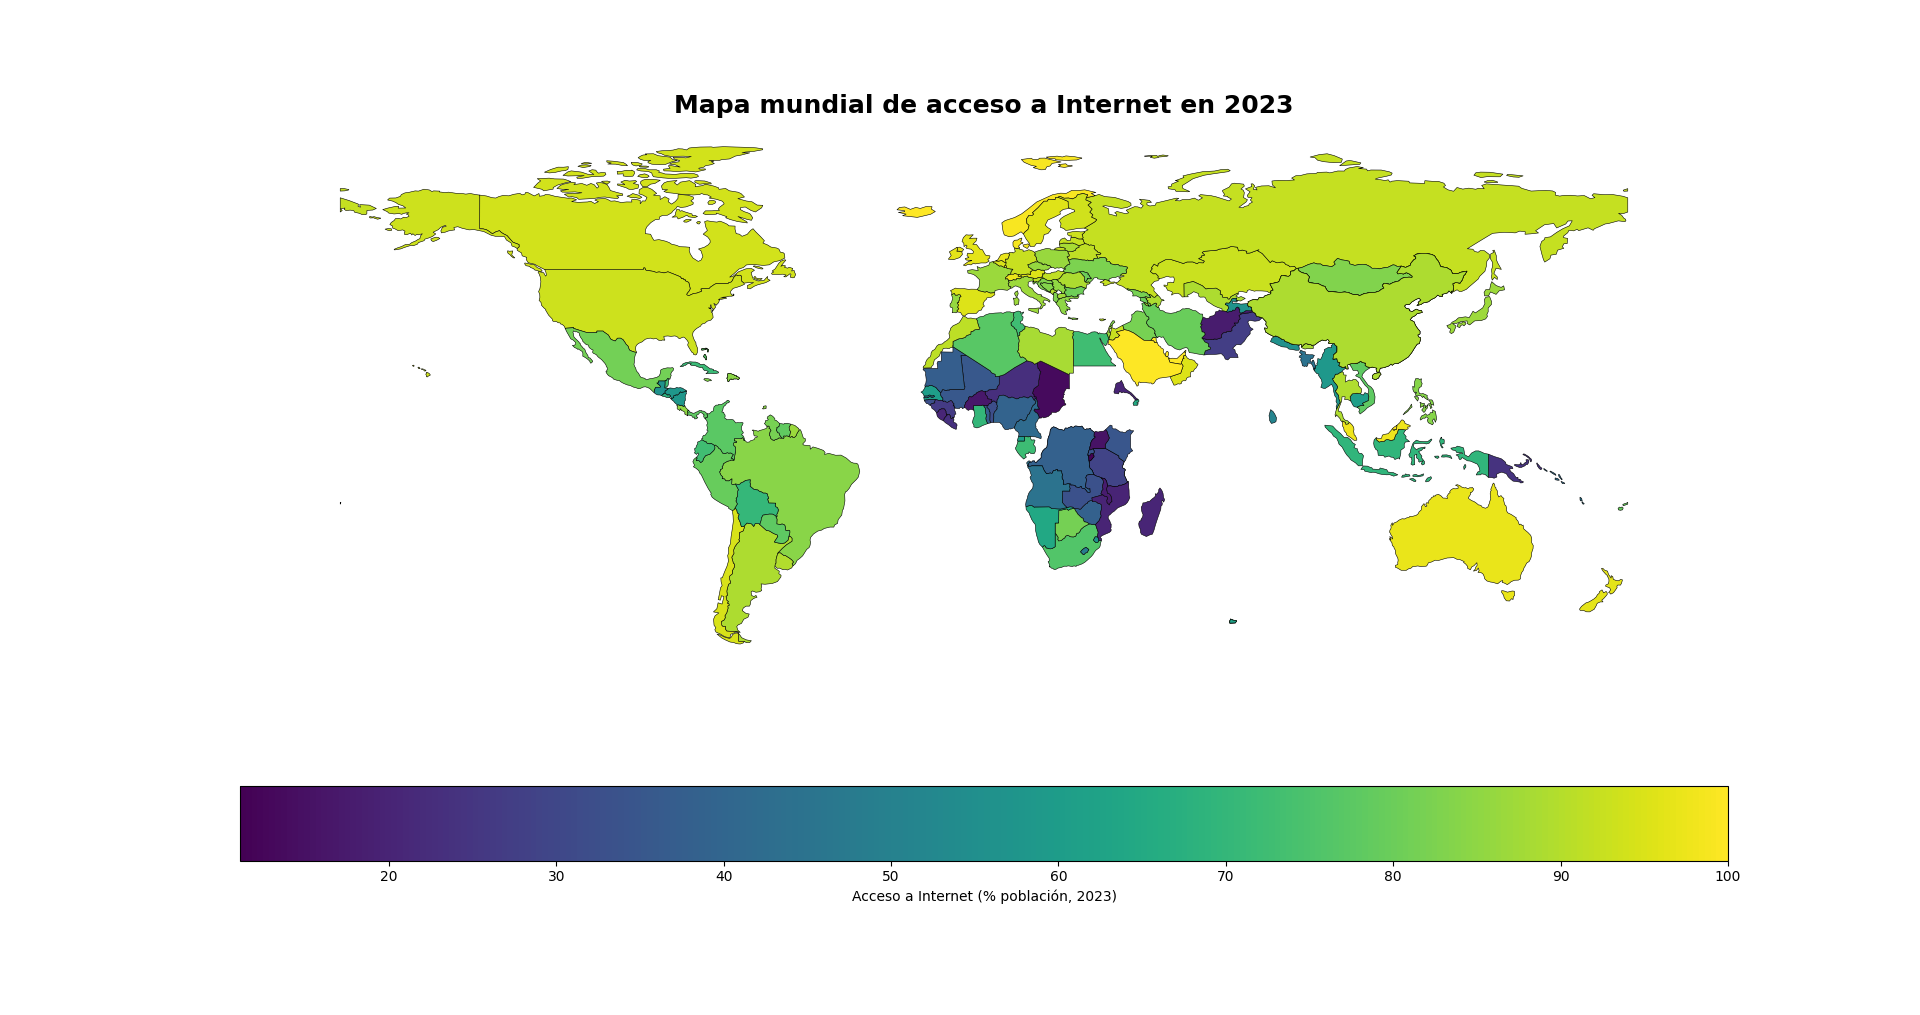
\includegraphics[width=0.85\textwidth]{images/Grafico_uso_de_internet_FC.png}
    \caption[1]{Fuente: Elaboración propia con datos de \href{https://data.worldbank.org}{World Bank} 
    (\url{https://data.worldbank.org/indicator/IT.NET.USER.ZS}).}
\end{figure}

\textbf{Conclusión:}
\begin{itemize}
    \item Muestra un panorama global del acceso digital: Europa, Oceanía y partes de Asia y América alcanzan más del 80\% de cobertura poblacional.
    \item África central y algunos países del sudeste asiático presentan niveles muy bajos (<40\%), lo que evidencia una brecha digital persistente.
    \item Países como Sudán, Congo o Yemen están en las zonas más oscuras del mapa, reflejando problemas estructurales en conectividad.
    \item Este mapa destaca diferencias regionales importantes que no necesariamente se reflejan en el gráfico de fibra óptica.
    \item Es una excelente forma de visualizar desigualdades sociales y tecnológicas a escala global.
\end{itemize}

\subsubsection*{Gráfico 2: Top 10 países con mayor porcentaje de fibra contratada}
\begin{figure}[H]
    \centering
    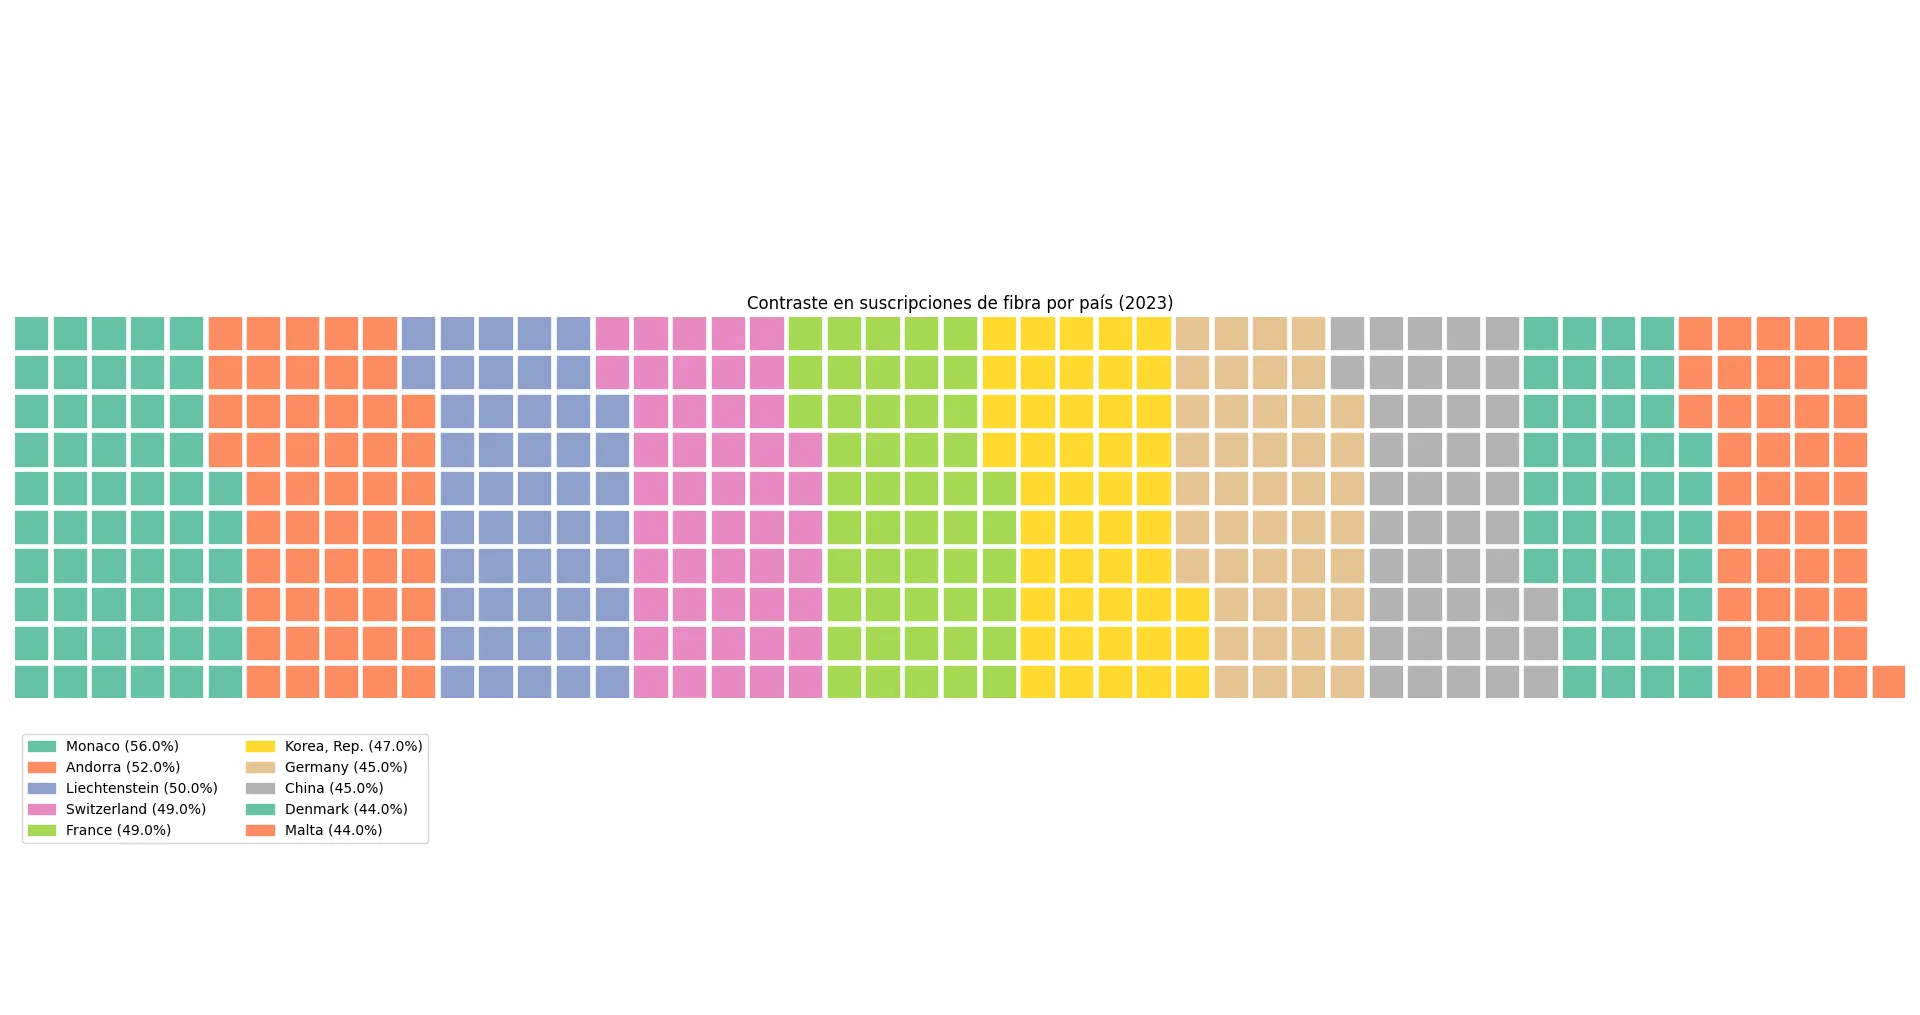
\includegraphics[width=1\textwidth]{images/Grafico_fibra_contratada_FC2.png}
    \caption[2]{Fuente: Elaboración propia con datos de \href{https://data.worldbank.org}{World Bank} 
    (\url{https://data.worldbank.org/indicator/IT.NET.BBND.P2}).}
\end{figure}

\textbf{Conclusión:}
\begin{itemize}
    \item Se observa que países como Mónaco (56\%), Andorra (52\%) y Liechtenstein (50\%) lideran la contratación de fibra en 2023.
    \item Son en general países pequeños, con economías desarrolladas y buena planificación urbana, lo que facilita la instalación de redes avanzadas.
    \item Países como China, Corea del Sur o Alemania también presentan cifras altas, pero no alcanzan el nivel de penetración de los primeros.
    \item El gráfico también muestra países con niveles más bajos, como Malta y Dinamarca (44\%), lo que sugiere diferencias internas incluso en regiones desarrolladas.
    \item Este tipo de visualización permite un contraste claro de adopción tecnológica y pone en evidencia el avance en infraestructura.
\end{itemize}


% ===================== JAVIER GÓMEZ =====================
\subsubsection*{Integrante 2: Javier Gómez}
Los criterios seleccionados por este integrante son los siguientes:
\begin{itemize}
    \item Criterio 1: Horas diarias en redes sociales.
    \item Criterio 2: Contratación de Telecomunicaciones.
\end{itemize}

\subsection{Justificación de Horas diarias en Redes Sociales}

Puede otorgar segmentación de audiencias, esto significa identificar que población tiene alto uso en redes sociales para lanzar campañas publicitarias en distintas redes sociales. \\
Desde otro ángulo podemos realizar un estudio si existe alguna relación entre la cantidad de horas diarias en el uso de \boldmath{RRSS} frente al rendimiento de estudiantes o salud mental de una persona.

\begin{itemize}
    \item Si estudiantes en un país pasan cierta cantidad de horas diarias en las redes, las instituciones educativas podrían implementar talleres sobre gestión del tiempo.
    \item Realizar estudio frente si existe relación entre las redes sociales y trastornos sicológicos.
\end{itemize}

\subsection{Justificación Contratación de Telecomunicaciones}
Revela qué compañías dominan la provisión de internet, destacando posibles monopolios u oligopolios, ej: Claro con el 45\% de contrataciones, lo que permite evaluar competencia real y calidad del servicio.

\begin{itemize}
    \item Muestra si los consumidores priorizan precios bajos, velocidad, cobertura u otros factores al elegir un proveedor
\end{itemize}
\subsection*{Gráfico 3: Horas diarias en redes sociales por país}
\begin{figure}[H]
    \centering
    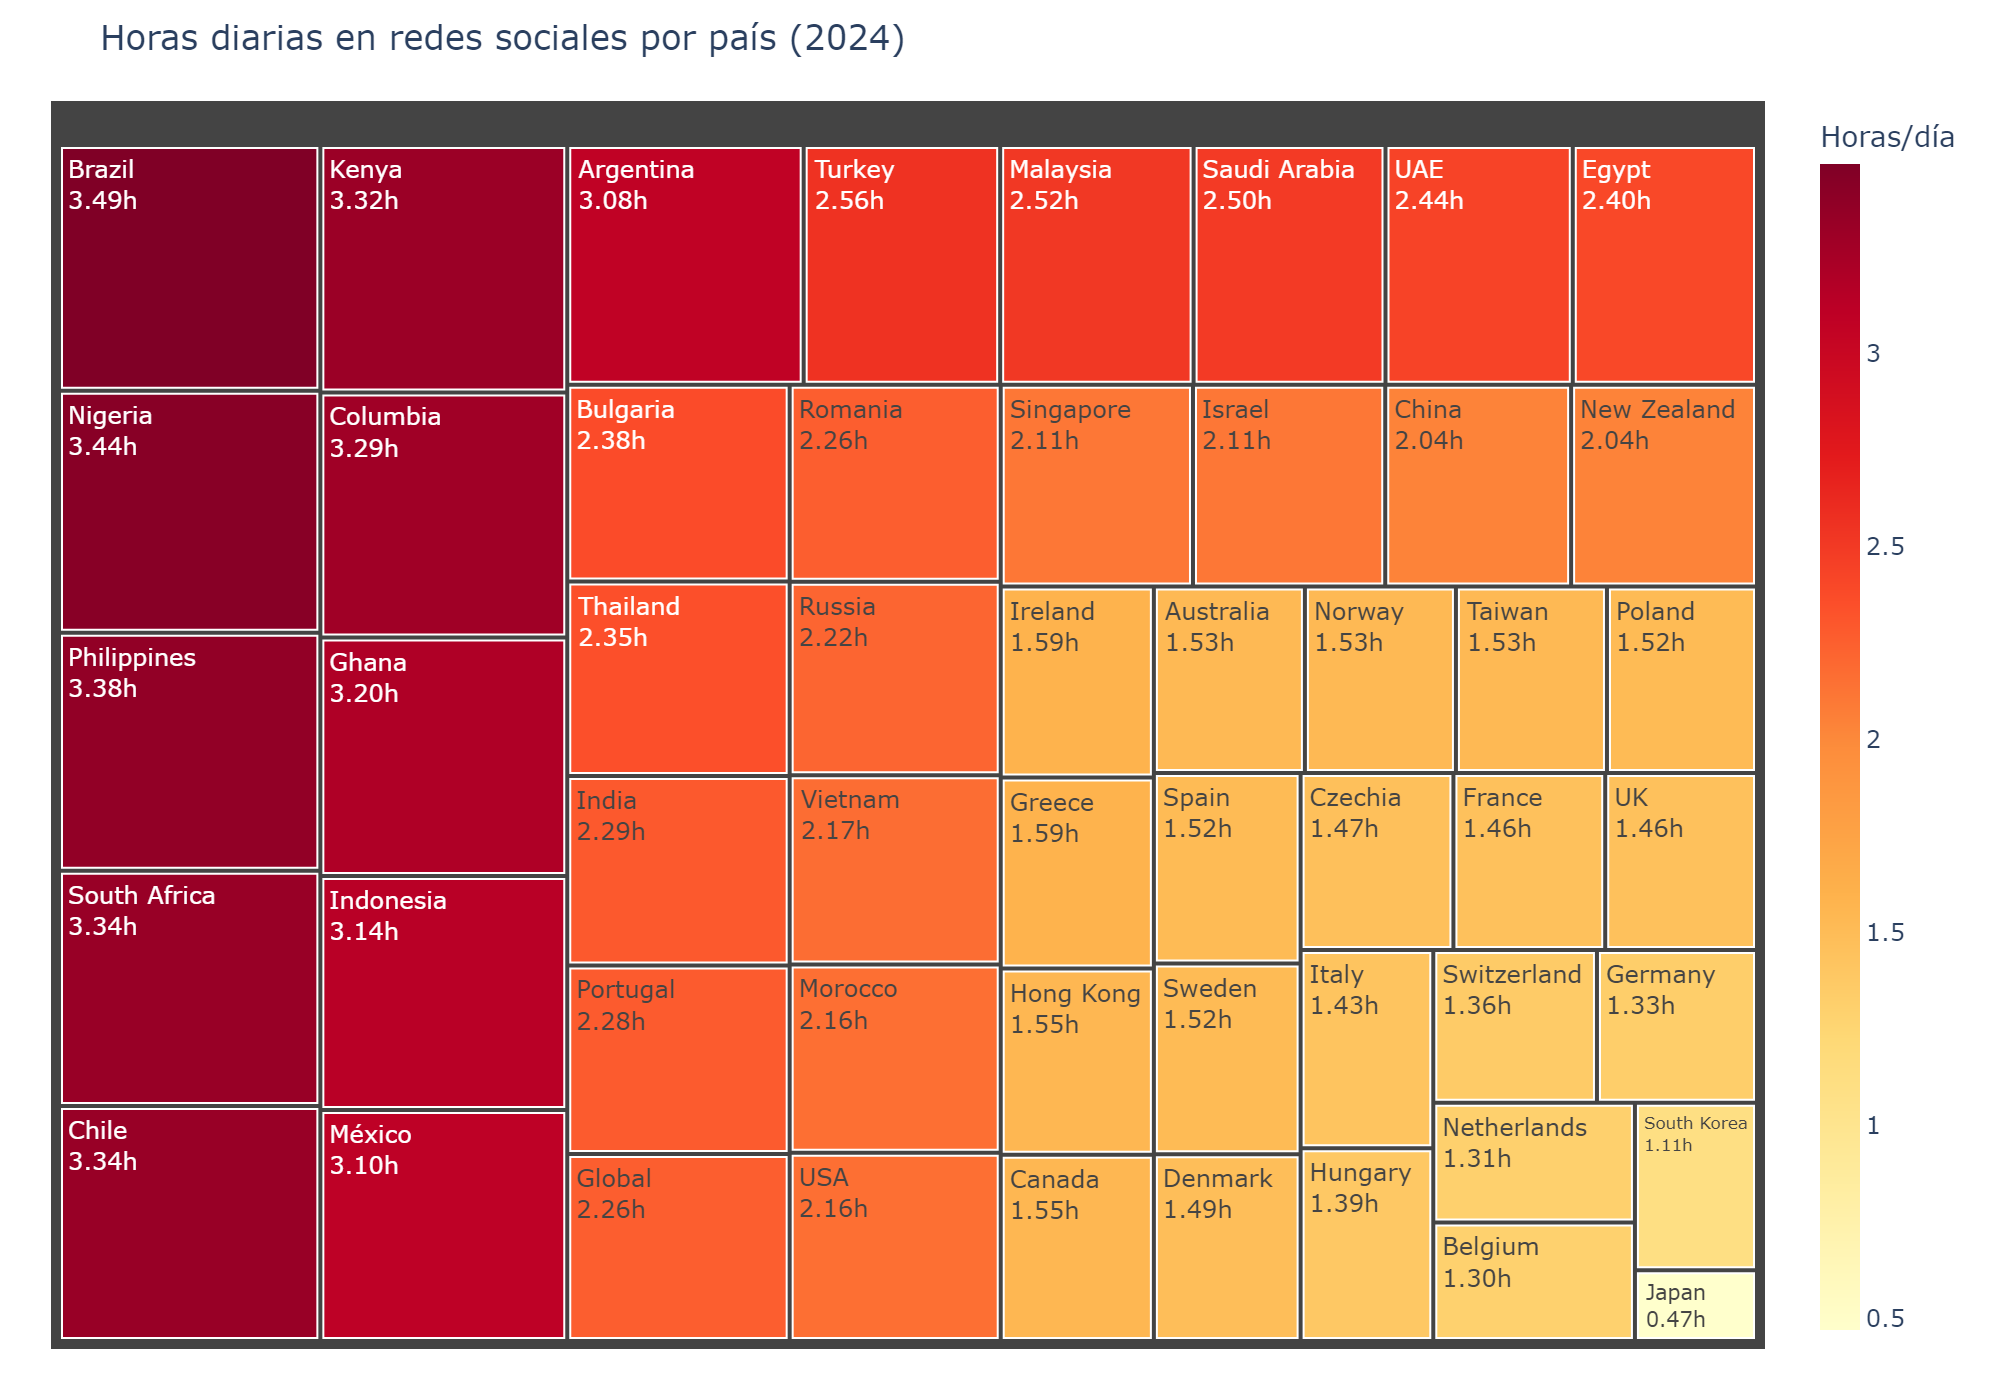
\includegraphics[width=0.85\textwidth]{images/graph1_JG.png}
    \caption{
        Fuente: Elaboración propia con datos de Statista (2024). 
        \textit{Promedio de minutos diarios de uso de redes sociales por los internautas en países seleccionados en el tercer trimestre de 2023}. 
        Recuperado de \url{https://www.statista.com/statistics/270229/usage-duration-of-social-networks-by-country/}
    }
\end{figure}


\subsubsection*{Conclusión}
Texto de conclusión específico para este gráfico. Analizar tendencias observadas y su relación con el impacto tecnológico en la vida cotidiana.

\subsection*{Gráfico 4: Evolución clientes por compañía de Telecomunicación}
\begin{figure}[H]
    \centering
    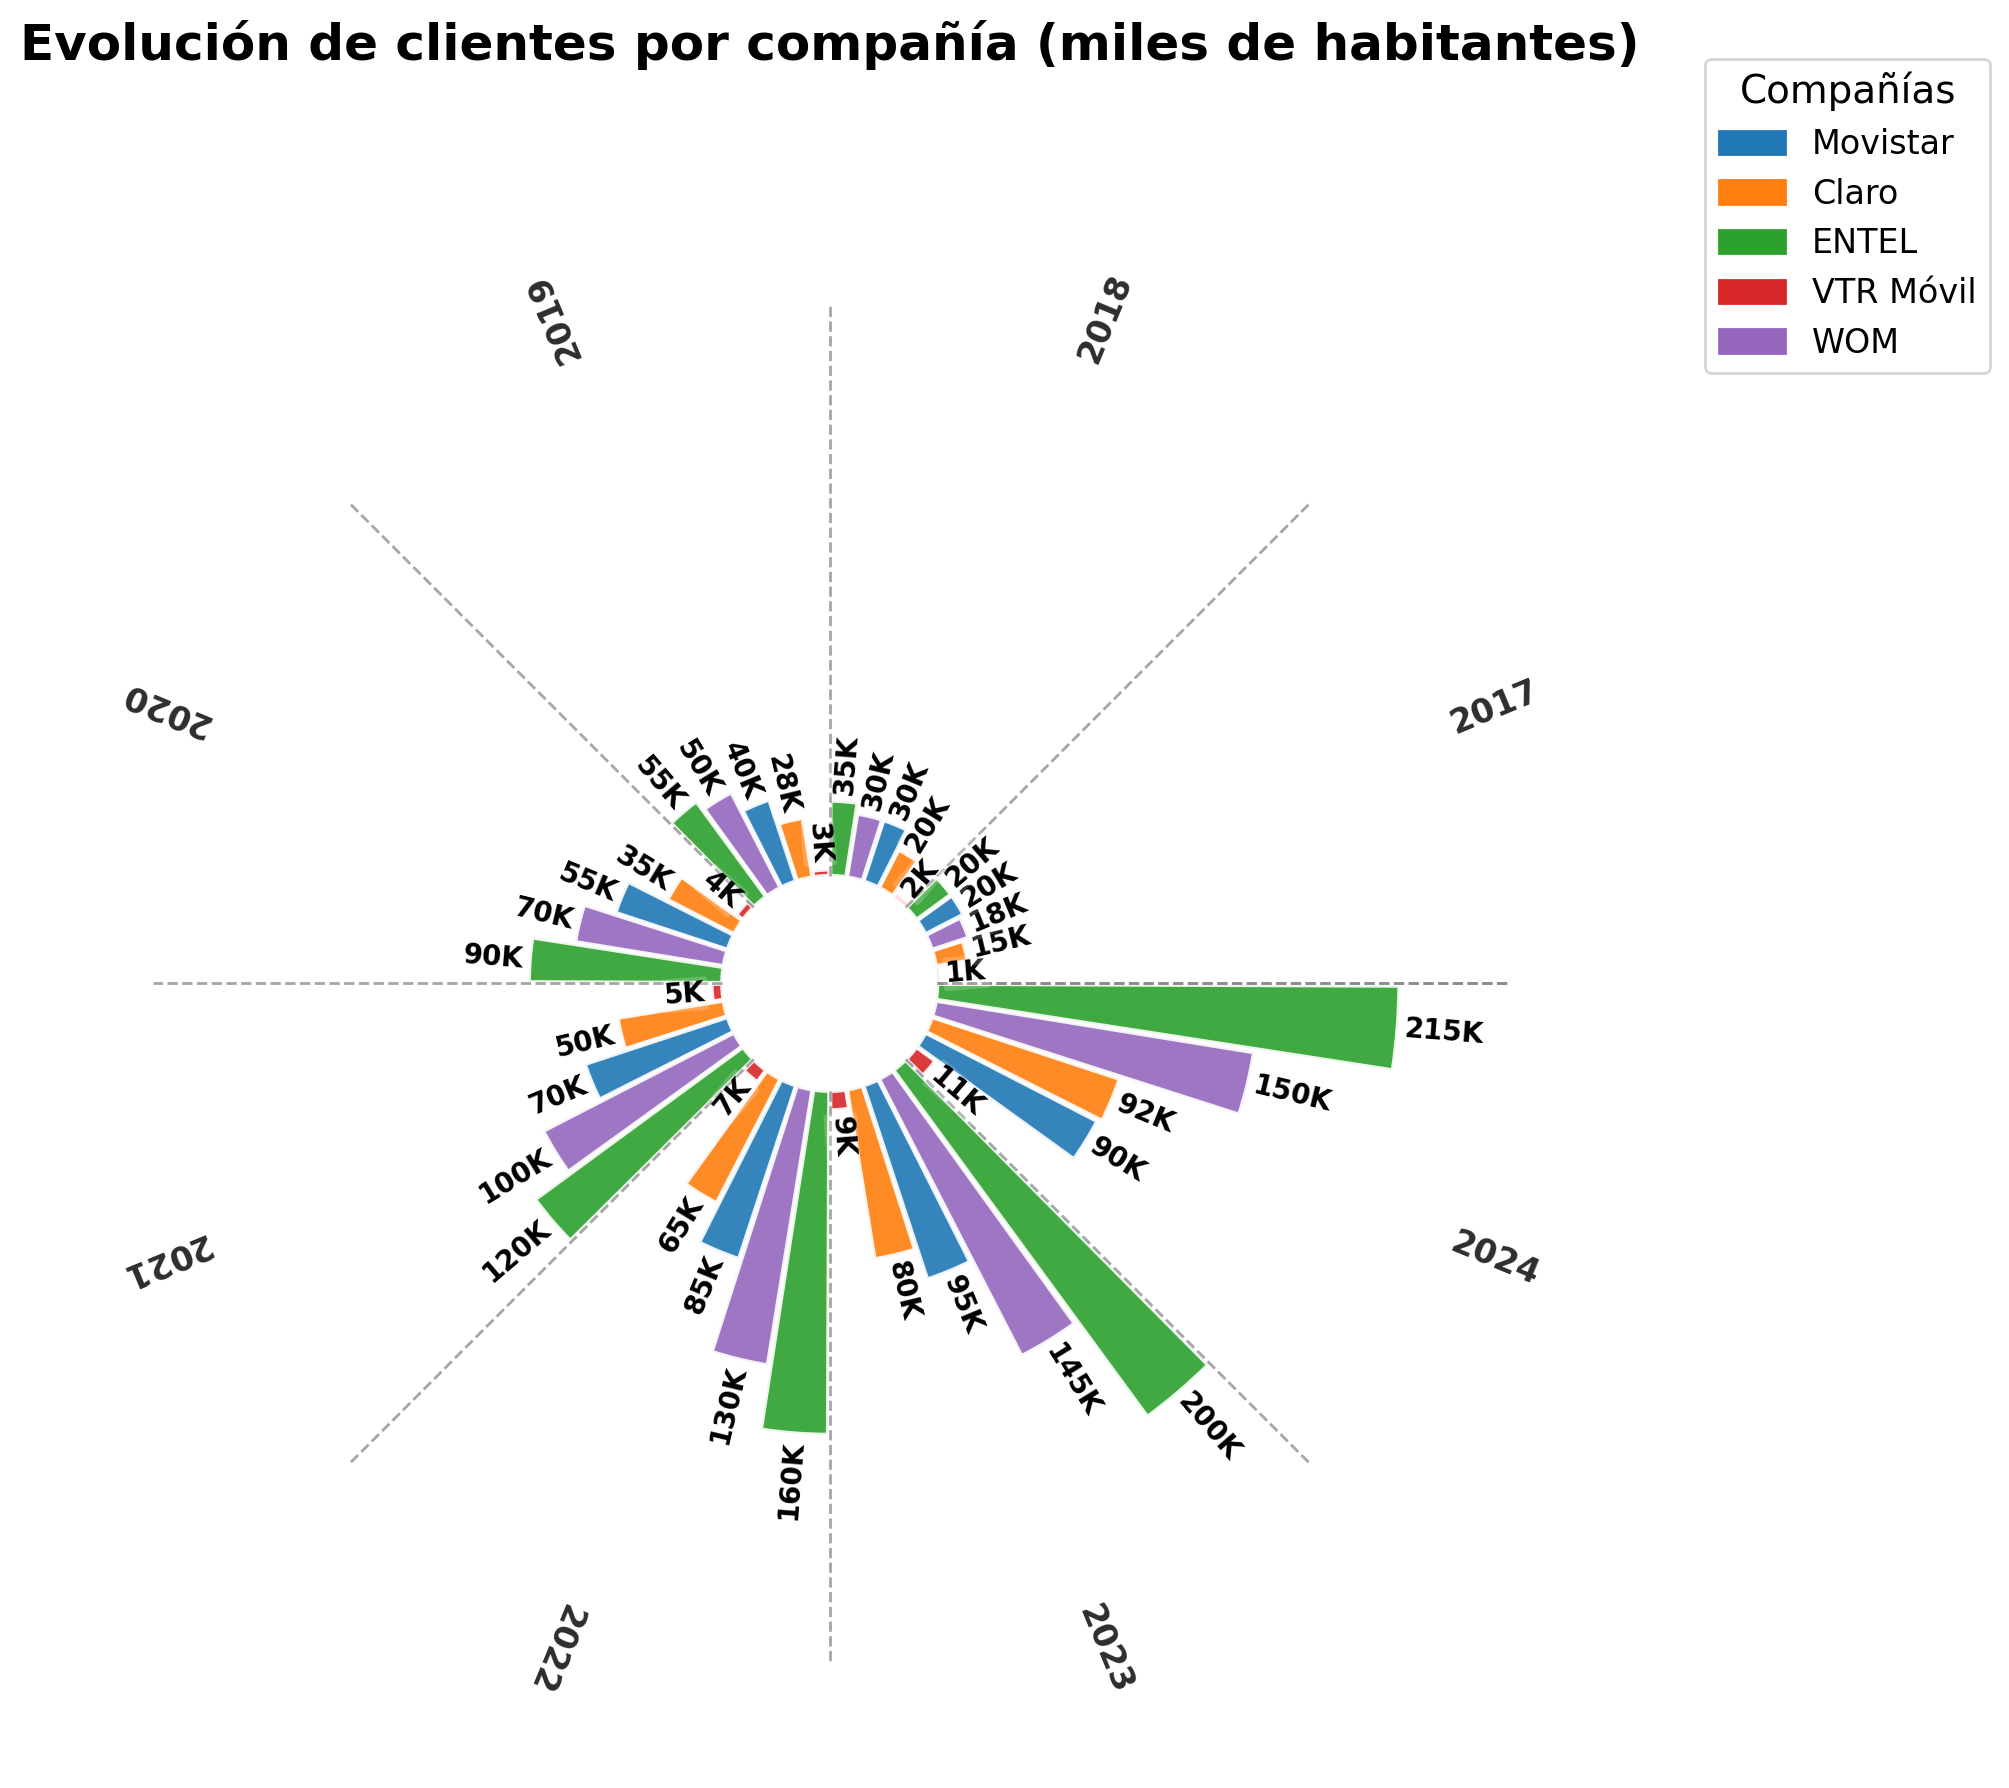
\includegraphics[width=0.85\textwidth]{images/graph2_JG.png}
    \caption{
        Fuente: Elaboración propia con datos de Subsecretaría de Telecomunicaciones (2025), 
        \textit{Informe del Sector Telecomunicaciones: Cierre 2024}, p. 13. 
        Disponible en \url{https://www.subtel.gob.cl/wp-content/uploads/2025/02/Informe_del_Sector_Telecomunicaciones_Dic24.pdf}
    }
\end{figure}

\subsubsection*{Conclusión}
Texto de conclusión específico para este gráfico. Analizar tendencias observadas y su relación con el impacto tecnológico en la vida cotidiana.



% ===================== MATÍAS ELGUETA (opcional) =====================
% Aquí puedes incluir una subsección para Matías Elgueta si va a desarrollar criterios o gráficos

% ---------------------------------------------------------------------------------
\section*{Conclusiones Generales}
\begin{itemize}
    \item Opcional**
\end{itemize}

\end{document}
